As seen from the data, the Extreme Learning Machines used 13 times more nodes on average when compared with the Back-Propagation model.
The number of nodes for the Back-Propagation model was chosen based upon the general rule of using $2n+1$ hidden-layer nodes for $n$ input nodes\ \citep{Tikhomirov:1991}.
Following this law, the number of nodes should have been $51$, but better generalization with the testing set was observed at $40$ nodes.
When a hidden layer size similar to  the Extreme Learning Machine model ($100$+ nodes) was chosen for stochastic gradient descent, the model performed worse than having fewer nodes even when the other parameters were adjusted to account for the increase.
In addition to worse performance, the training time increased substantially as the number of hidden layer nodes increased.

Although the Extreme Learning Machines used more nodes, their training time and mean-squared error were significantly lower when compared with the Back-Propagation model.
The Extreme Learning Machine model also had a higher hit or miss success rate.
The averaged results in the table within section 5 show that Extreme Learning Machines could forecast both types of hit or miss ratios for each stock better than the Back-Propagation model.
Extreme Learning Machines forecasted an average of 73.5\% and 68.4\% of the time correctly while the Back-Propagation model forecasted an average of 64.2\% and 50.4\% of the time correctly for types 1 and 2, respectively.

\begin{figure}
	\begin{center}
	\resizebox{\textwidth}{!} {
	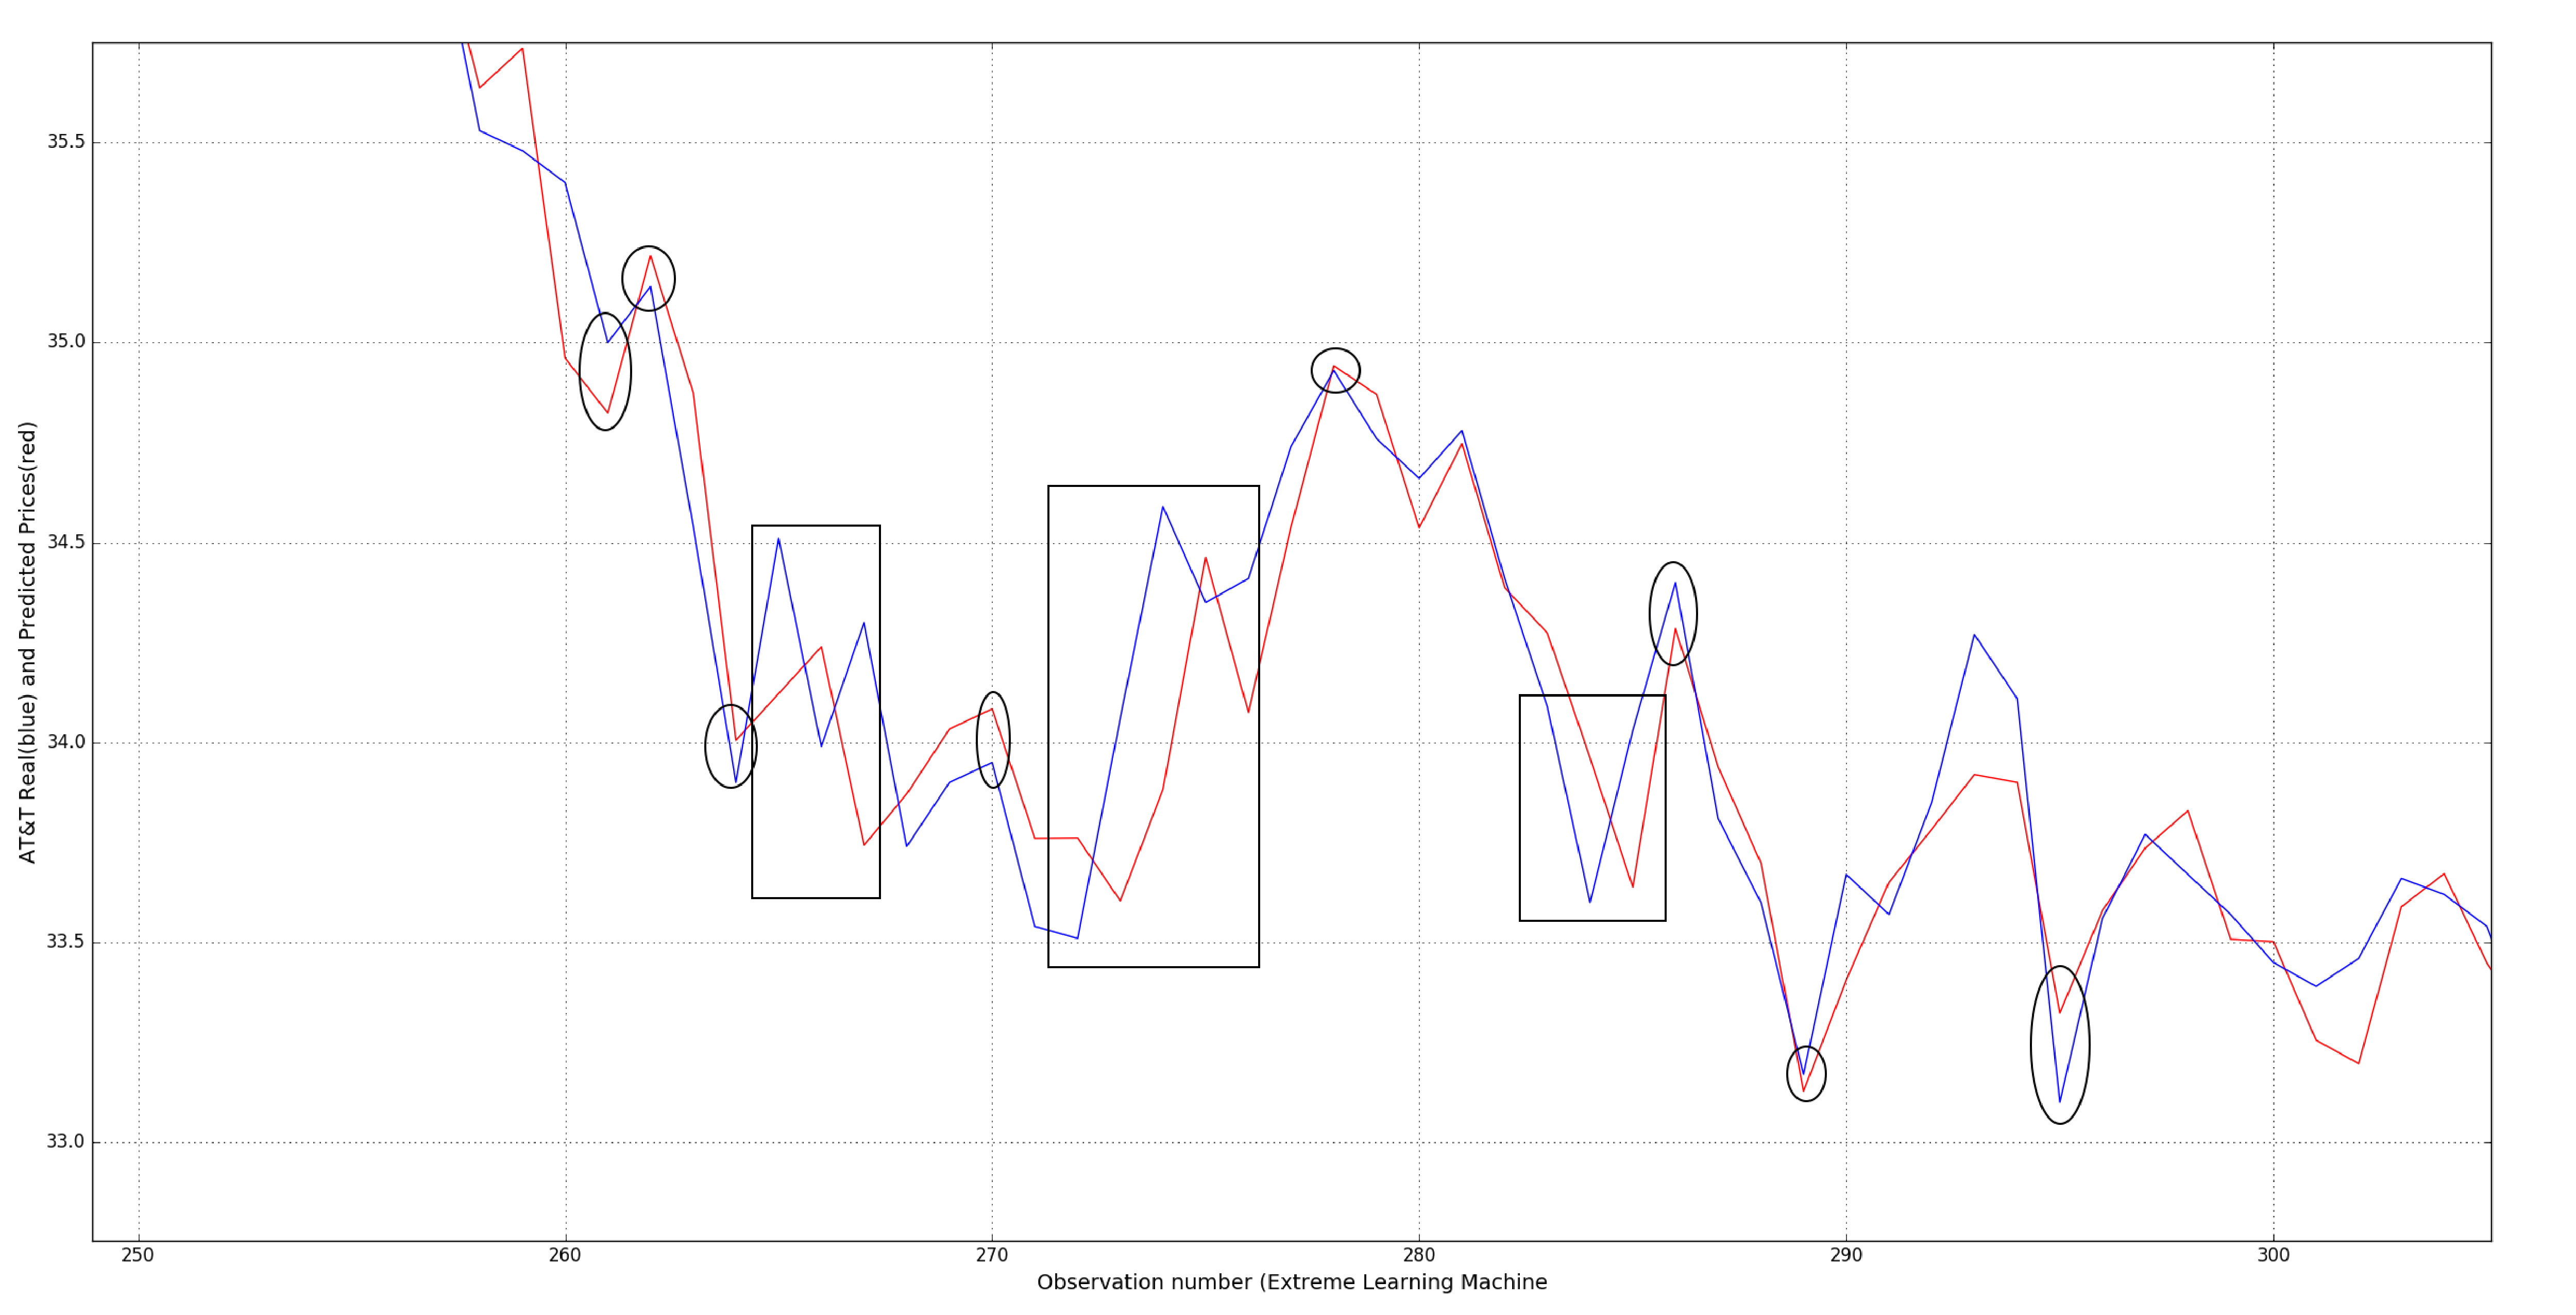
\includegraphics{images/projecting_prices}}
	\caption{ Black Rectangles: Forward Projected forecasts, Black circles: Correct inflection. }
	\label{projected_prices}
	\end{center}
\end{figure}

Projecting data is one of observed patterns that happened for both models.
In this situation, the predicted closing prices (red) look like the forward projection of the real closing prices (blue) within graph~\ref{projected_prices}.
The instances of these projections are outlined with black rectangles.
In these situations, the models found a very simple method of producing a close approximation and lowering the training error, which impacted the results of testing.
The model is reacting to the stock changes instead of reacting with the stock changes.
The graph above was an arbitrary choice, and these patterns were seen infrequently throughout the testing data.

The forward projection of previous closing prices might not be a problem.
Even though both of these models' weights were optimized with different methods, both of these models exhibit this pattern.
This may indicate that the issue is difficult to resolve and is a results of the training process or noisy data.
This could also be a consequence of using Artificial Neural Networks for financial forecasting because neural networks are unpredictable when classifying noisy data.

After projecting previous days forward, both methods were seen to adjust their predictions to correctly forecast inflection points as shown by the black circles.
From the previous section, the Extreme Learning Machine model showed that it predicted the sign of change and inflection points with high accuracy, so on average, the model outperforms the Efficient Market Hypothesis.
The Back-Propagation model was less successful with forecasting the sign of change and inflection points.

\begin{figure}
	\begin{center}
	\resizebox{\textwidth}{!} {
	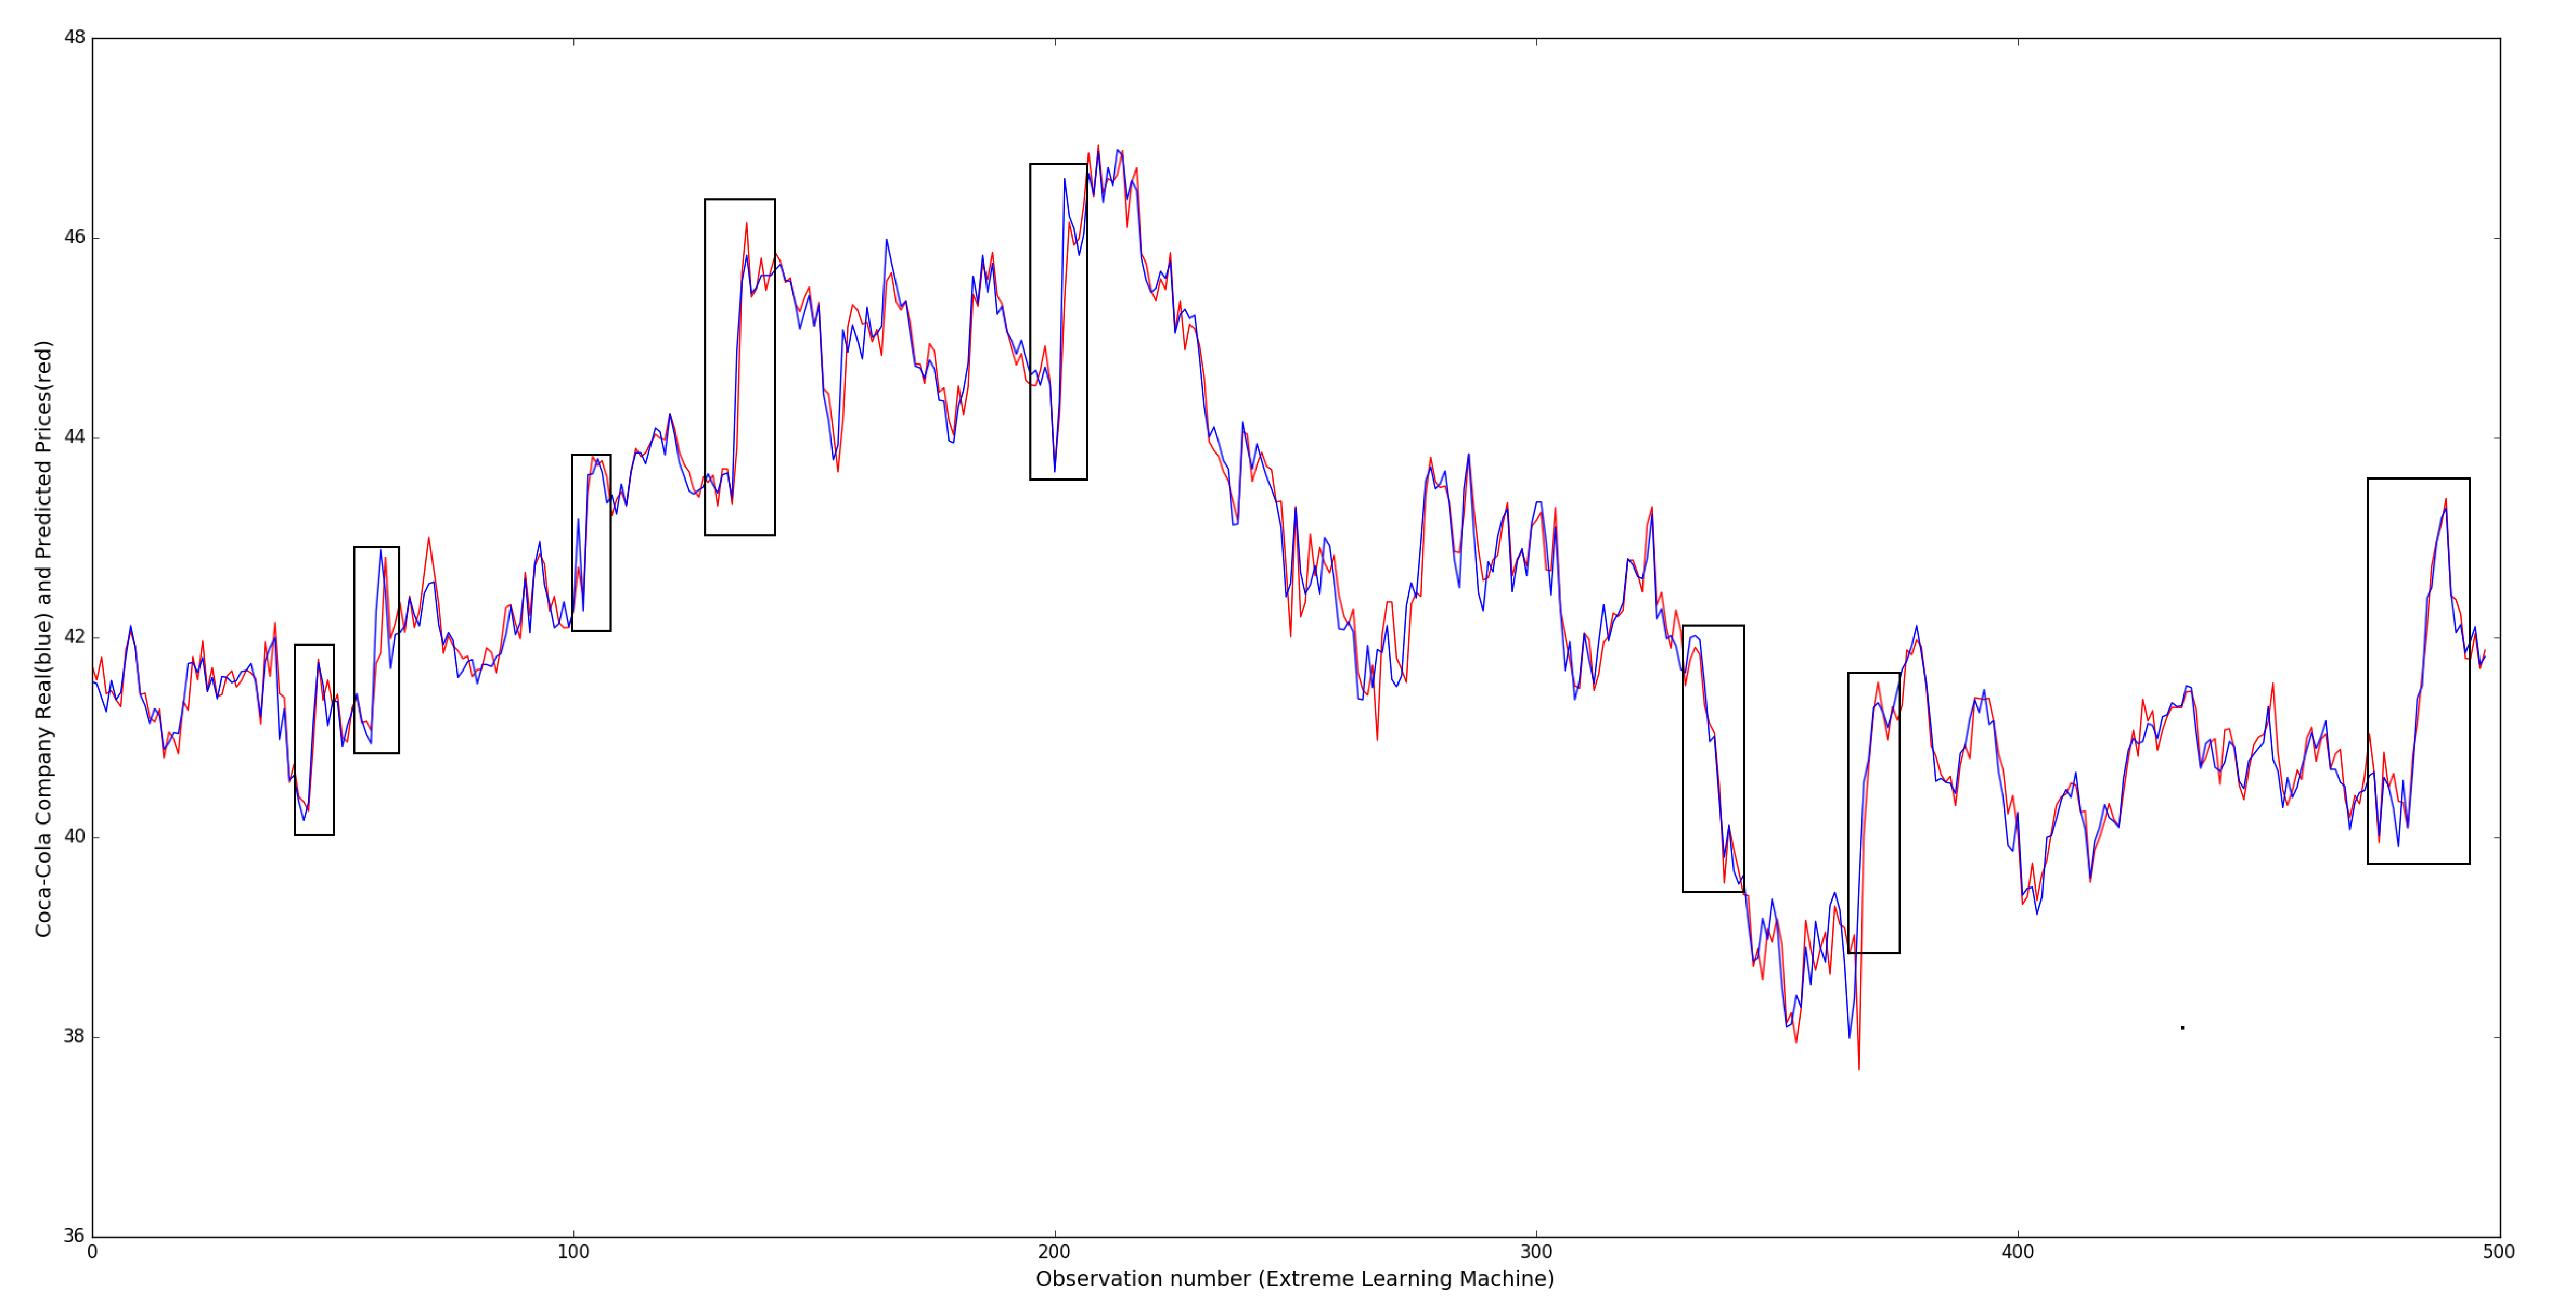
\includegraphics{images/threshold_response}}
	\caption{ Black Rectangles: Forecasted threshold responses }
	\label{threshold_responses}
	\end{center}
\end{figure}

Both models performed well with forecasting threshold responses as in graph~\ref{threshold_responses}.
Thresholds exist in markets where the market begins to quickly change in price.
For the five testing stocks, both models forecasted the same pattern for these rapid price changes.
The Extreme Learning Machine model tended to over predict and under predict these changes less than the Back-Propagation model.
Both models became more proficient at forecasting threshold responses after the data sets were preprocessed using min-max linear scaling.

% Conclusion